\documentclass{achemso}
\usepackage[utf8]{inputenc}
\usepackage[dvipsnames]{xcolor}
\usepackage{amsmath}
\usepackage{multirow}
\definecolor{richelectricblue}{rgb}{0.03, 0.57, 0.82}
\newcommand{\vv}[1]{{\textbf{\textcolor{red}{Venkat: #1}}}}
\newcommand{\ab}[1]{{\textbf{\textcolor{ForestGreen}{Alec: #1}}}}
\newcommand{\abattention}[1]{{\textbf{\textcolor{Orange}{Alec: #1}}}}
\newcommand{\lf}[1]{{\textbf{\textcolor{richelectricblue}{Leif: #1}}}}
\newcommand{\ssri}[1]{{\textbf{\textcolor{cyan}{SS: #1}}}}
\graphicspath{ {./Figures/} }

\title{Batteries Required to Electrify Commercial Aircraft}
\author{Alexander Bills}
\affiliation{%
 Department of Mechanical Engineering, Carnegie Mellon University, Pittsburgh, Pennsylvania 15213\\
}

\author{William Leif Fredericks}
\affiliation{%
 Department of Mechanical Engineering, Carnegie Mellon University, Pittsburgh, Pennsylvania 15213\\
}

\author{Shashank Sripad}
\affiliation{%
 Department of Mechanical Engineering, Carnegie Mellon University, Pittsburgh, Pennsylvania 15213\\
}

\author{Madalsa Singh}
\affiliation{%
 Department of Mechanical Engineering, Carnegie Mellon University, Pittsburgh, Pennsylvania 15213\\
}

\author{Venkatasubramanian Viswanathan*}
\affiliation{%
 Department of Mechanical Engineering, Carnegie Mellon University, Pittsburgh, Pennsylvania 15213\\
}
\email{venkvis@cmu.edu}
\date{February 2019}

\begin{document}


%%%%%INTRODUCTION%%%%%%%%

\section{Introduction}

Electric aircraft have generated an enormous amount of interest following the success of the electrification of passenger vehicles. Over 5 million passenger electric vehicles have been sold\textbf{cite}, and there have been numerous announcements regarding electrification of SUVs, pick-up trucks and other light commercial vehicles, which represent the majority of the passenger automotive market today. \vv{cite relevant things here.} However, while electrification of ground vehicles is well underway, electrification of aircraft is still in its infancy. Announcements have been made regarding electric vertical takeoff and landing (eVTOL) aircraft by companies including Uber \textbf{cite}, Airbus \textbf{cite}, and others. In a recent viewpoint, we identified the challenging battery requirements faced by eVTOL aircraft, reiterating  the obvious importance of specific energy (defined as the energy available per unit mass) and identifying the importance of power limitations and thermal management requirements during take-off and landing. \vv{cite} While eVTOL aircraft represent a new market for electrification, electrifying existing commercial aircraft could reduce the environmental impact of the transportation segment as a whole. Currently, commercial aircraft represent 9\% of the carbon emissions from transportation, and even more of the warming effect as a result of Aircraft-Induced cloud contrails\textbf{cite}. Efforts are underway towards the development of electric commercial aircraft\vv{cite Zunum, Wright, Pratt, etc}. In addition, countries (e.g. Norway) are intending to partially or fully electrify their fleet over the next few decades.   Further, the world's largest seaplane operator, Harbor Air, announced their intention to electrify their fleet.\vv{cite} However, despite all this excitement, numerous technological challenges remain; the chief among them is the performance metrics required of batteries to electrify commercial aircraft.  Several analysis have presented a comprehensive system-level perspective on the challenges and have identified sub-system component targets.\vv{Cite Epstein, Barrett etc}  In this viewpoint, we primarily focus on developing a detailed understanding of the performance metrics required of batteries to electrify the commercial aviation market and a discussion of possible approaches towards meeting these metrics.

One major challenge in identifying battery pack requirements is the wide variety of commercial aircraft on the market and the associated uncertainty due to this heterogeneity. As will become evident from analysis, we divide commercial aircraft into three categories: regional, narrow body, and wide body. Regional aircraft typically fly short missions, about 500 Nautical Miles (NMi) and carry low passenger loads (30-75), while wide body aircraft carry high passenger loads (200-400) and fly much longer missions ($>2000$ NMi). Narrow body aircraft fall somewhere in between, carrying medium passenger loads and flying medium ranges ($\sim$1000 NMi).

%----Intro up to here------%

%----Methods --- 
\section{Methods}

In the course of a mission, aircraft take off, climb to their cruising altitude, cruise to their destination, descend to near ground level, then land. Takeoff and landing are neglected in this study because their energy use is low due to their relatively short duration in flight. Commercial aircraft also must have some emergency reserve energy storage for contingencies such as diversions or aborted landings. The FAA requires that aircraft must be able to abort a landing, climb to normal cruising altitude, fly to an alternate airport 200 nautical miles away, and loiter for 45 minutes. \textbf{Cite} 30\% state of charge has been proposed as an alternative to the extant FAA commercial reserve. In \textit{(Supplementary Information)} we show that the choice between these two possible reserves does not substantially impact the feasibility of the aircraft; we use the 30\% state of charge reserve for simplicity. 

To estimate the energy requirement, we use a flight dynamics model which takes an integrated "First Principles" energy and power estimation approach, similar to the one we used to analyze the electrification of light commercial vehicles, \cite{sripad2017evaluation}, semi-trucks, \cite{guttenberg2017evaluating,sripad2017performance}, and eVTOLs \textbf{Cite Leif}. Four forces act on an aircraft in flight: thrust (force generated by the propulsion system), drag (aerodynamic force opposite to the direction of motion), weight (gravitational force), and lift (aerodynamic force normal to the wings). Power is a function of the geometry and operating conditions of the aircraft, including instantaneous velocity relative to the surrounding airmass (V), zero lift drag coefficient ($C_{D0}$), propulsive efficiency($\eta_{prop}$), mechanical efficiency($\eta_{mech}$), wingloading (S), aspect ratio, and climb or descent angle ($\gamma$).  We assume that at any point in flight, thrust equals drag and lift equals weight. To calculate power at any point during flight,  thrust is multiplied by the velocity, resulting in Equation \ref{eqn:masterPower}. To calculate energy required by the aircraft, the instantaneous power, given in Equation \ref{eqn:masterPower}, is integrated over the duration of the mission. 

\begin{equation}\label{eqn:masterPower}
    \centering
    \mathrm{P = \frac{\frac{1}{2}\ V^3\ S\ C_{D0}\ \rho + \frac{2\ K\ W^2}{\rho\ V\ S} + W\ V\ sin(\gamma)}{\eta_{prop}\ \eta_{mech} }}
\end{equation}

Calculating the performance of prospective aircraft is complicated by the considerable uncertainty of the parameters in Equation \eqref{eqn:masterPower}. Velocity (V) and induced drag correction factor (K) are dependent on other parameters; they are derived in the supporting information. This leaves the zero-lift drag coefficient ($C_{D0}$), propulsive efficiency($\eta_{prop}$), mechanical efficiency($\eta_{mech}$), Wingloading (S), and aspect ratio\ab{We never really show what aspect ratio is, is this a problem?} to be estimated based on existing aircraft of each size. We will discuss methods of dealing with this uncertainty later in this paper. Uncertainty in the mass of aircraft components is also a concern. Rather than estimating aircraft component weights (which is outside the scope of this paper), we  employ the ratio (known as the empty weight fraction) of the weight of the aircraft mass without batteries and payload to the total mass. Table 1 contains the upper limit, lower limit, and nominal values of the parameters for each category of aircraft. 


\begin{table}[]
\centering
\resizebox{0.99\textwidth}{!}{%
\begin{tabular}{|l|p{1cm}|p{1cm}|p{1cm}|p{1cm}|p{1cm}|p{1cm}|p{1cm}|p{1cm}|p{1cm}|p{1cm}|p{1cm}|p{1cm}|}
\hline
\multirow{2}{*}{Aircraft Class} & \multicolumn{3}{c}{MTOM (Kg)}                                                                   & \multicolumn{3}{c}{Aspect Ratio}                                                                & \multicolumn{3}{c}{Wing Loading (Kg/m\textasciicircum{}2)}                                      & \multicolumn{3}{c}{Drag Coefficient}                                                            \\
                                & \multicolumn{1}{l}{Lower Limit} & \multicolumn{1}{l}{Upper Limit} & \multicolumn{1}{l}{Nominal} & \multicolumn{1}{l}{Lower Limit} & \multicolumn{1}{l}{Upper Limit} & \multicolumn{1}{l}{Nominal} & \multicolumn{1}{l}{Lower Limit} & \multicolumn{1}{l}{Upper Limit} & \multicolumn{1}{l}{Nominal} & \multicolumn{1}{l}{Lower Limit} & \multicolumn{1}{l}{Upper Limit} & \multicolumn{1}{l}{Nominal} \\
Regional                        & 11,500                          & 52,290                          & 50,000                      & 7.62                            & 12.6                            & 12                          & 292                             & 565                             & 400                         & .014                            & .024                            & .018                        \\
Narrow Body                     & 44,225                          & 123,380                         & 100,000                     & 7.79                            & 10.5                            & 11                          & 434                             & 789                             & 500                         & .014                            & .024                            & .018                        \\
Wide Body                       & 142,882                         & 447,696                         & 250,000                     & 7.99                            & 10.1                            & 10                          & 504                             & 808                             & 600                         & .014                            & .024                            & .018                       
\end{tabular}}
\end{table}
%--------Analysis-------------%
\section{Analysis}


\subsection{Analysis Method 1: Parameter Uncertainty}
To mitigate uncertainty in the parameters for Equation \eqref{eqn:masterPower}, we conducted a monte carlo simulation by sampling each of the parameters in table 1 from a uniform distribution. The mission for this analysis (i.e. range and payload) was defined a priori.  The range for regional aircraft was defined as 350 NMi, for narrow body aircraft, it was 500 NMi, and for wide body aircraft, it was 2000 NMi. These were chosen as the minimum practical ranges for each class. The passenger count for regional aircraft was 75, for narrow body aircraft was 150, and for wide body aircraft was 300. The take off mass for regional aircraft was 50000 Kg, for narrow body aircraft was 100000 Kg, and for wide body aircraft was 250000 Kg. Figure 1 shows the resulting histogram of specific energy.

\begin{figure}[htp]
\centering

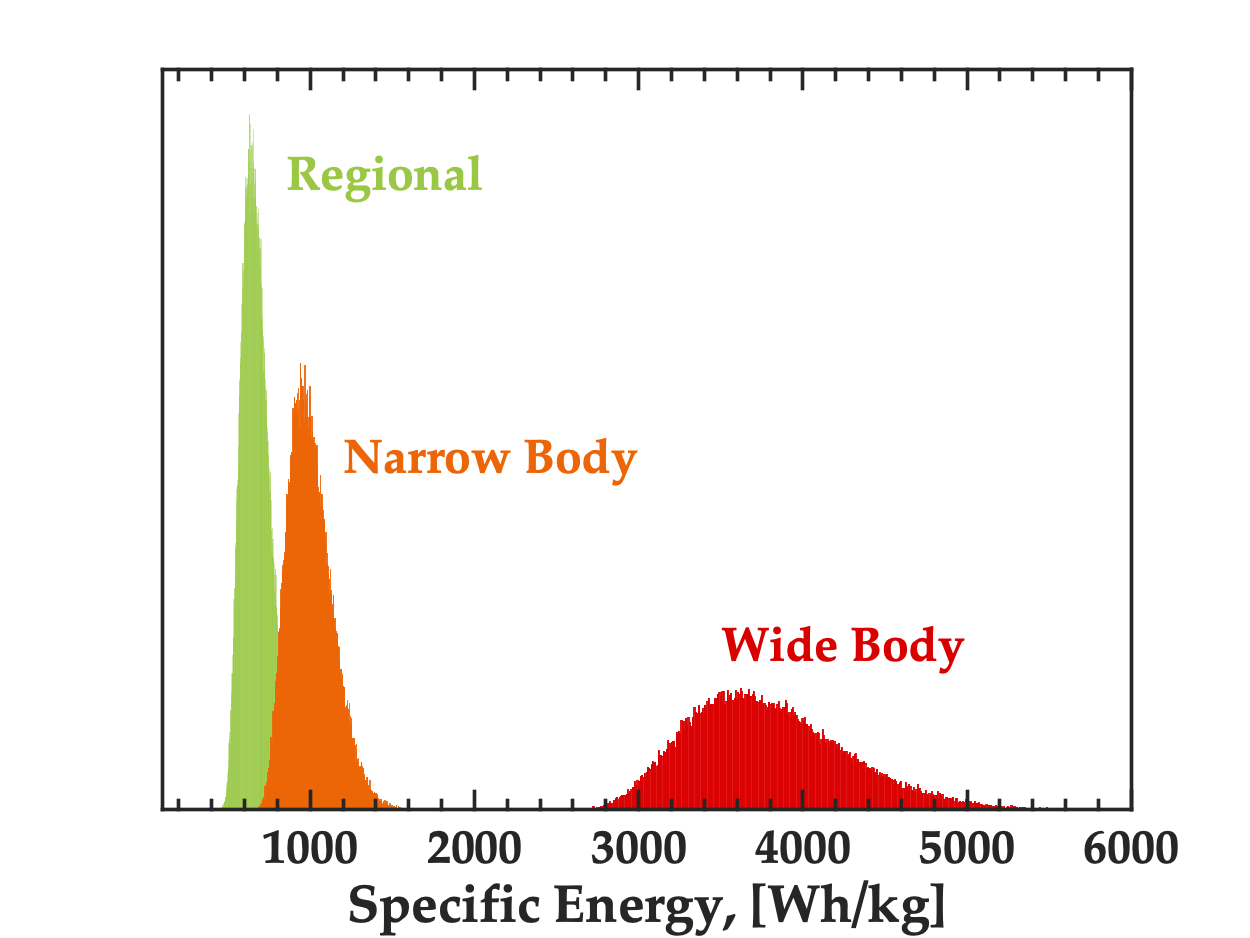
\includegraphics[width=0.6\textwidth]{Figures/histograms.png}

\caption{Histograms of specific energy for regional, narrow body, and wide body aircraft. This figure clearly illustrates the uncertainty resulting from the parameter uncertainty in each aircraft class. The wide body case in particular is extremely uncertain.}
\label{fig:figure1}

\end{figure}

The distribution of required specific energy for a regional aircraft has lower and upper bounds of around 475 Wh/Kg and 725 Wh/Kg. While these bounds are relatively high, the mode of the distribution is located around 550 Wh/Kg. For a narrow body aircraft, the lower and upper bounds are around 650 Wh/Kg and 975 Wh/Kg, respectively. Its mode lies around 750 Wh/Kg. For the wide body aircraft, the lower bound is around 2000 Wh/Kg and the upper bound is around 3500 Wh/Kg. The mode for the wide body aircraft is located around 2500 Wh/Kg. These data indicate the wide disparity between the performance metrics required of batteries to electrify regional aircraft and the performance metrics required to electrify larger and longer range aircraft. 

Satisfying these predefined mission requirements does not a guarantee that an aircraft is commercially feasible. Small aircraft, such as regional and some narrow body aircraft, often have cruise ranges that are much lower than their maximum range. However, large aircraft often use a much larger proportion of their maximum range in a typical flight. For example, the airbus A319, a small narrow body aircraft, is most likely to fly a range of around 299 Km in cruise, and the distribution of its flights are skewed towards the lower end of its range of ranges. On the other hand, a wide body aircraft, such as the Boeing 777 nearly always flies towards the high end of its range, with a mode cruise length of 4843 Km. 

\subsection{Analysis Method 2: Contours and Max PNMi}

To analyze the commercial feasibility of a prospective electric aircraft, we will study the mission capabilities as a function of specific energy. All parameters in Equation \eqref{eqn:masterPower} are set to their nominal values. We will use the number of passengers multiplied by the aircraft range (PNMi) as a figure of merit to study system feasibility at each specified EWF and SE. To ensure that the algorithm does not converge to a corner case (e.g. no passengers and extreme long range or high passengers and extreme short range), we subtract a minimum range and passengers. The minima are different for each class and are set by studying historical aircraft of each class. We then plot the passengers from the aircraft with the highest PNMi at each design point on figure 2 and the range from that design point on figure 3. Regional aircraft are first able to satisfy the minimum requirements for this analysis at a specific energy of around XXX. Narrow body aircraft are first able to satisfy the minimum requirements at a specific energy of around YYY. Wide body aircraft require a specific energy of at least ZZZZ. 

\begin{figure}[htp]
\centering
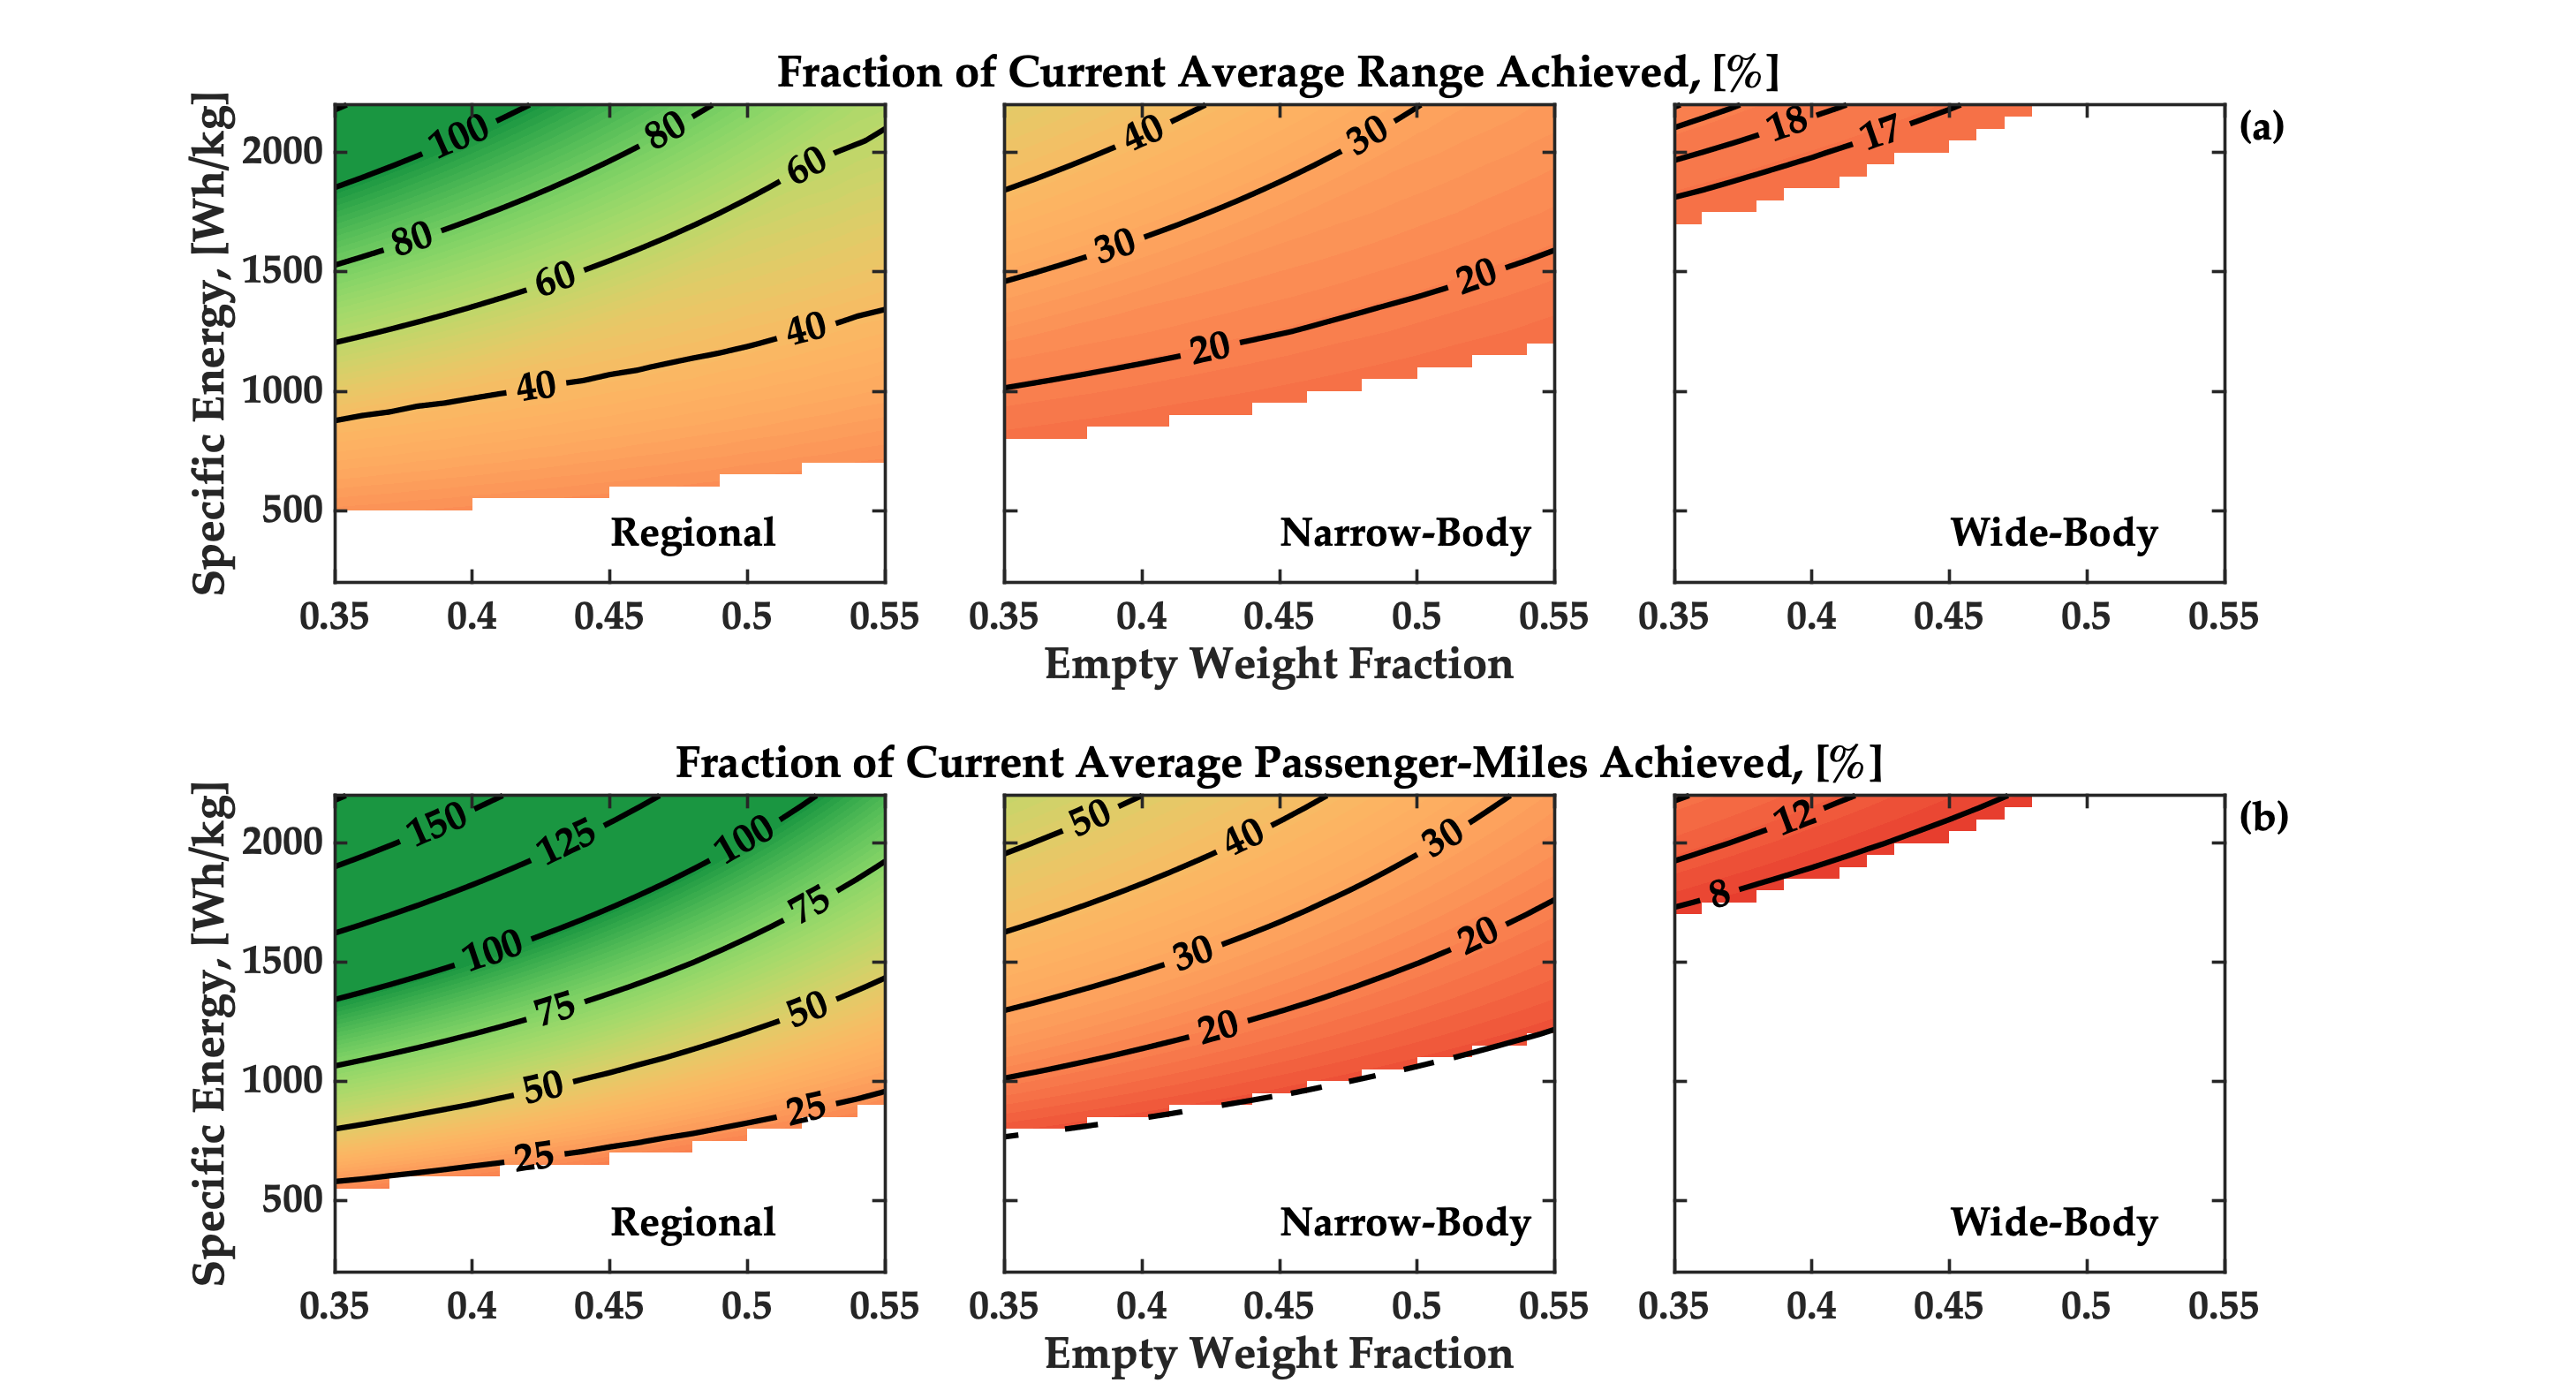
\includegraphics[width=\textwidth]{Figures/contours.png}\hfill
\caption{Range and Passengers for regional, narrow body, and wide body aircraft at optimal PNMi}
\label{fig:figure2}
\end{figure}

In any case, the specific energy required of a wide body aircraft is much greater than that of a regional aircraft. This effect is largely due not to the larger size of the aircraft, but rather to the increased range. To illustrate this effect, consider the power profiles of each of the classes of aircraft for representative ranges flown by each (Figure 4). While the size of the aircraft results in the higher power at each point, the energy required to fly the ranges flown by aircraft (the area beneath the curve) increases even more as a result of the increased range. 

\begin{figure}[htp]
\centering
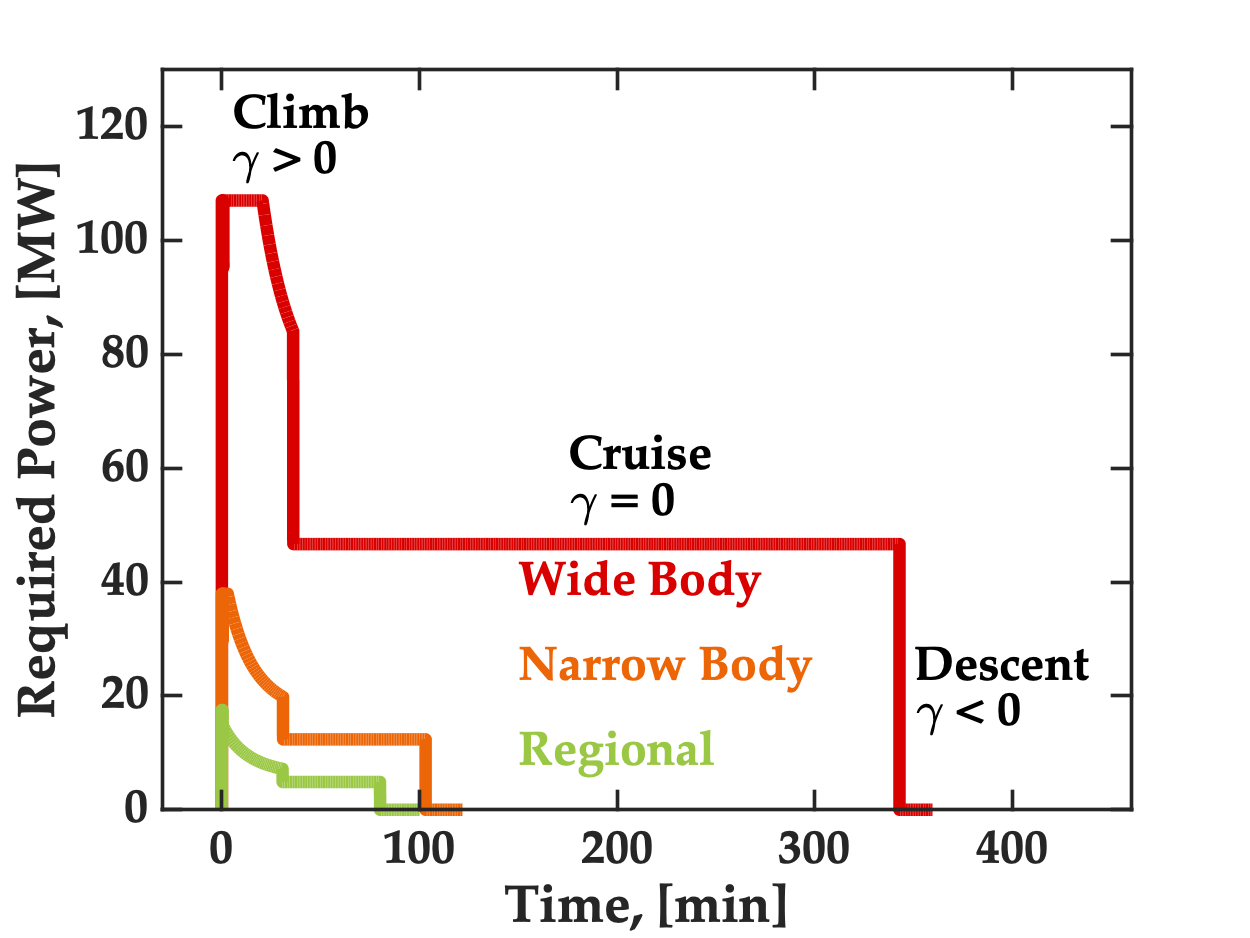
\includegraphics[width=0.6\textwidth]{Figures/powerprofiles.png}
\caption{Aircraft Power Profiles, along with conditions of flight in each segment. This figure illustrates the scaling challenges inherent in electric flight; as MTOM increases, the typical use case range also increases, causing a massive increase in the total energy needed}
\label{fig:figure4}
\end{figure}

To find which parameters most affect the performance metrics required for an electric aircraft, a sensitivity analysis was performed. The result is shown in Figure 5, where the specific energy is plotted as a function of percentage change from the mean for each parameter to carry out the mission described above.  In each case, the combined efficiency is the most important factor, followed closely by EWF, Drag Coefficient and aspect ratio. Wing loading has a much lower effect on the requirements than do the other parameters. It should be noted here that extensive trade studies are often done in aircraft conceptual design and the effects of these parameters on anything other than power and energy requirements are outside the scope of this paper and were not studied.
\begin{figure}[htp]

\centering
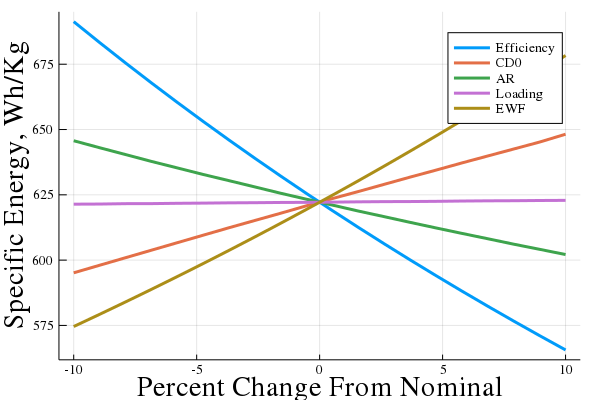
\includegraphics[width=.3\textwidth]{Figures/RJ_Sensitivity.png}\hfill
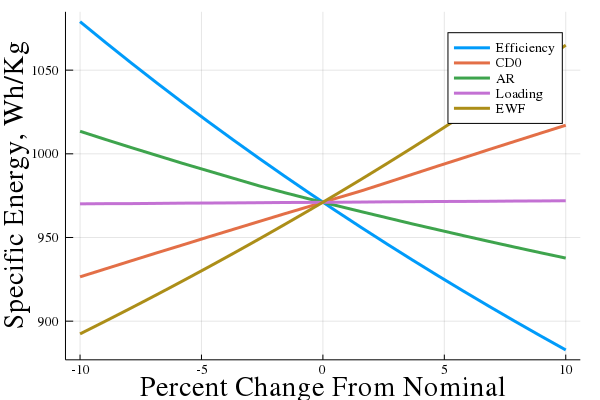
\includegraphics[width=.3\textwidth]{Figures/NB_Sensitivity.png}\hfill
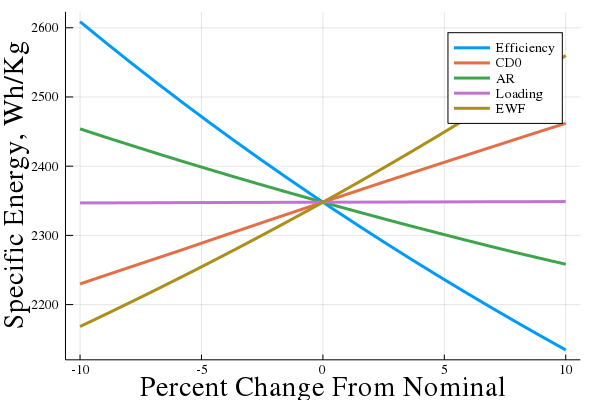
\includegraphics[width=.3\textwidth]{Figures/WB_Sensitivity.png}

\caption{Sensitivity Analysis for regional, narrow body, and wide body aircraft}
\label{fig:figure5}

\end{figure}

\subsection{Discussion of batteries required to meet these requirements, along with discussion of discharge rates}
% \abattention{SHASHANK}
The discussion thus far has not explicitly examined battery chemistries and materials needed to achieve the specific energy requirements of the three segments of electric aircraft.  For the purpose of this study, we categorize batteries into current commercial Li-ion batteries, `future Li-ion batteries' including concepts such as silicon or Li-metal based anodes and solid state electrolytes, and `beyond Li-ion batteries' which include chemistries such as Li-S and Li-O$\mathrm{_2}$. \textbf{(cite)} The specific energy of current generation Li-ion batteries has steadily increased by XXX over the last XXX years \textbf{(cite the Srinivasan paper)} with projected practical maximum SE values at the cell-level of about XXX and about XXX at the pack-level with Graphite-based anodes and layered oxide cathodes. Silicon anodes are projected to provide up to ... and Li-metal would result in an increase of about ... , however, there is uncertainty in the power capability of these systems. Notwithstanding it should be noted that, if the specific energy criterion is not met by a specific battery system, it is not considered for further analysis. The two conversion chemistries considered here are Li-Sulfur and Li-Oxygen/Air ...

(In the flight modeling section), we examined regional and narrow-body aircraft within the limits of 200 Wh/kg and 1,200 Wh/kg while wide-body aircraft were examined under the limits of 200 and 2,200 Wh/kg. 

....Figure (\ref{fig:ragone}) shows the reduction the specific energy

\begin{figure}[h!]
\centering
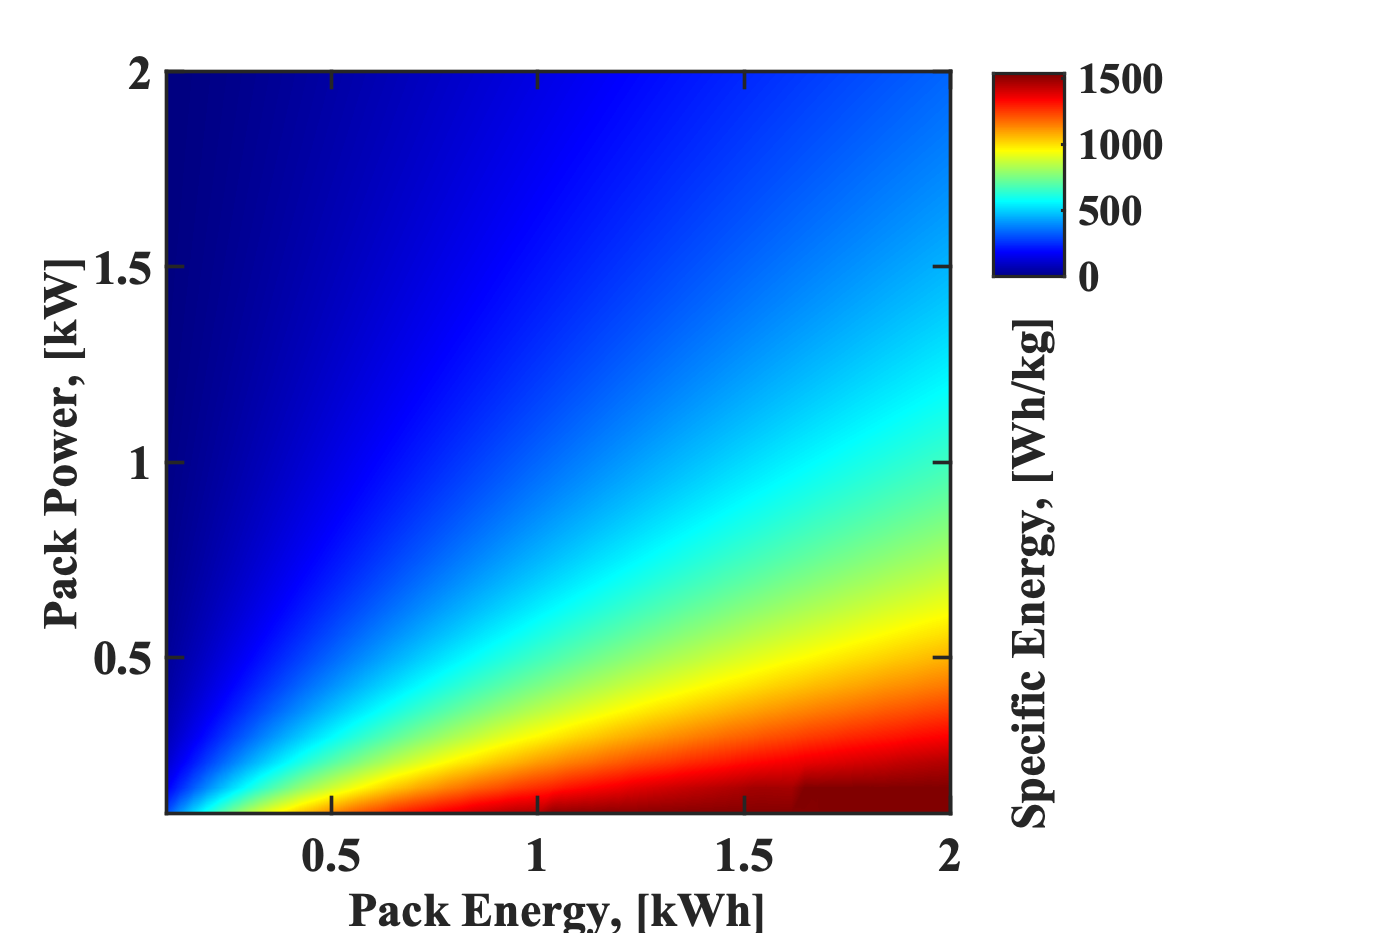
\includegraphics[width=0.6\linewidth]{ragone.png}
\caption{Pack specific energy of Li-air open systems for different pack-level energy and power metrics.}
\label{fig:ragone} 
\end{figure} 


\subsection{Future Work, including BLI and Emissions and Money and Stuff}

Aviation's contribution to anthropogenic climate change is not fully understood, however aviation seems to contribute to it in a few ways. Conventional jet engines emit greenhouse gases such as carbon dioxide, water vapor, nitrous oxides, sulfates and soot when they burn jet fuel. The contrails emitted by aircraft also are a major cause of warming. According to a XXXX paper \textbf{cite whatever madalsa wanted to cite here}, aircraft induced cloudiness causes more than 50\% of the aviation-derived radiative forcing, which directly induces warming in the upper troposphere. While we, as others, found that the barriers to electrifying large aircraft on long flights are quite high, electrifying smaller aircraft offer some real opportunities, and the chance to remove up to 15\% of their carbon emissions from the environment. Additionally, electrifying aircraft would eliminate aircraft induced cloudiness, one of the major contributors to anthropogenic climate change from aviation. 



% Determining the aviation sector’s contribution to anthropogenic climate change is a work-in-progress. One major segment studies greenhouse gas emissions – carbon dioxide, water vapour, nitrous oxides, sulphates, soot - released from burning jet fuel; while others have studied the impact of aircraft-induced cloudiness on the large-scale climate system. There is also a growing body of literature looking at air quality impacts due to fuel burn during aircraft landing and take-off (LTO) for various segments of aviation (NOT ELABORATING AS LTO ENERGY USE IS IGNORED IN OUR TEXT but climate/AQ benefits are plenty) \textbf{(cite lead study, air pollution around airports study, NOx study)}. Electrification of aviation nullifies all three during operation.\\
% While there are challenges to electrify large long-range aircraft at the current state of battery technology \textbf{(cite eipstein)}, smaller aircraft (\textbf{ENTER PAX VALUE OR RANGE DEPENDING ON CONCLUSIONS FROM OUR PAPER)} can reduce carbon emissions by 15\% \textbf{(cite barrett, also added in eipstien}) can serve as starting points for decarbonization of aviation.  \\
% Beyond carbon emissions, it is important to look at the benefits of electrification of aviation by complete removal of Aircraft Induced Cloudiness (AIC) – short term condensation trails (contrails) and long-lived Cirrus homogenitus \textbf{(cite nature paper)}. Within climatic uncertainties, Aircraft induced cloudiness accounts for more than 50\% share in aviation-derived radiative forcing which directly induces warming in upper troposphere. Electrification of aviation would enable rapid and complete mitigation of AICs.

%%%%%%%Batteries

\end{document}
